\documentclass{beamer}

\usepackage{amsmath}

\begin{document}
%--------------------------------------------------------- %
\begin{frame}
\huge
\[ \mbox{Discrete Mathematics: Set Theory}\]
\[ \mbox{Using Venn Diagrams}\]
\Large
\[ \mbox{www.Stats-Lab.com}\]
\[ \mbox{Twitter: StatsLabDublin}\]
\end{frame}
\begin{frame}
\Large
Shade in the following areas on Venn diagrams.
\begin{itemize}
\item[(a)] $A^\prime\; \cup\; B$

\item[(b)] $A \cap\; B^\prime\;$

\item[(c)] $(A \cap\; B)^\prime\;$

\item[(d)] $A^\prime\; \cup\; B^\prime\;$

\item[(e)] $(A \cup\; B)^\prime\;$

\item[(f)] $A^\prime\; \cap\; B^\prime\;$

\end{itemize}
\end{frame}

\begin{frame}
\Large
\[(a) \;\; A^\prime \; \cup\; B\]
\begin{figure}
\centering
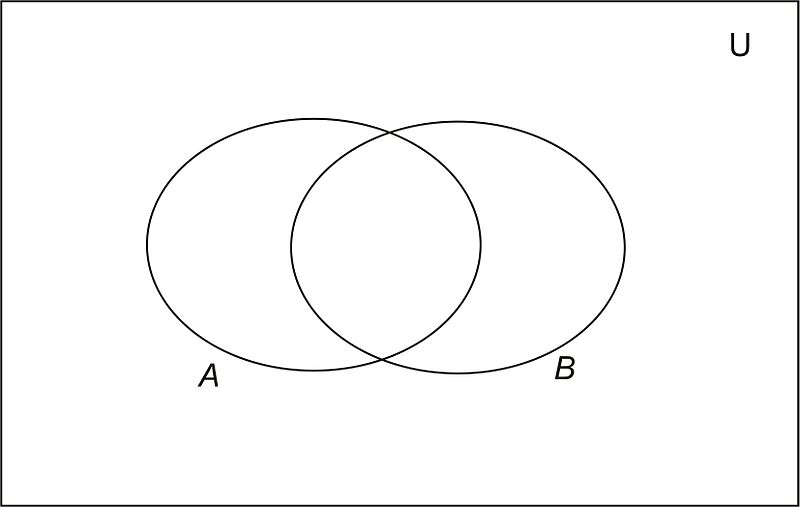
\includegraphics[width=0.8\linewidth]{Venn}
\end{figure}
\end{frame}
%--------------------------------------------------------- %
\begin{frame}
%Question 2
\Large
\[(b) \;\; A \cap\; B^\prime\;\]
\begin{figure}
\centering
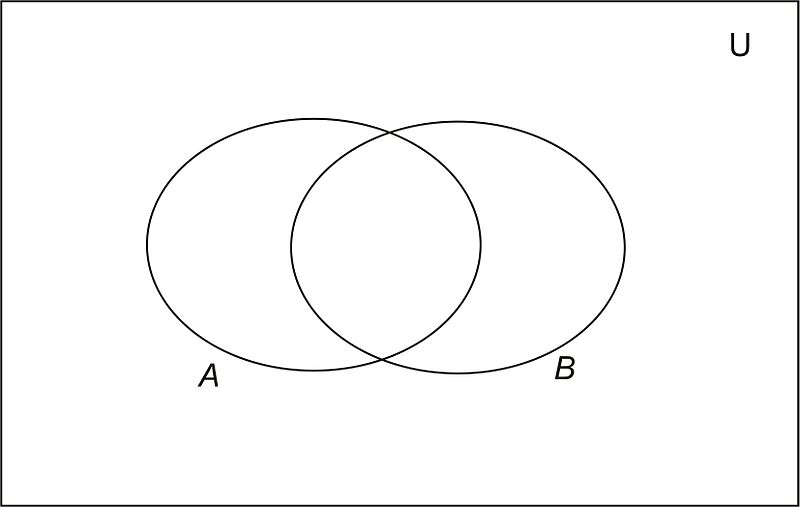
\includegraphics[width=0.8\linewidth]{Venn}
\end{figure}
\end{frame}
%--------------------------------------------------------- %
\begin{frame}
%Question 3
\Large
\[(c) \;\; (A \cap \; B)^\prime\;\]
\begin{figure}
\centering
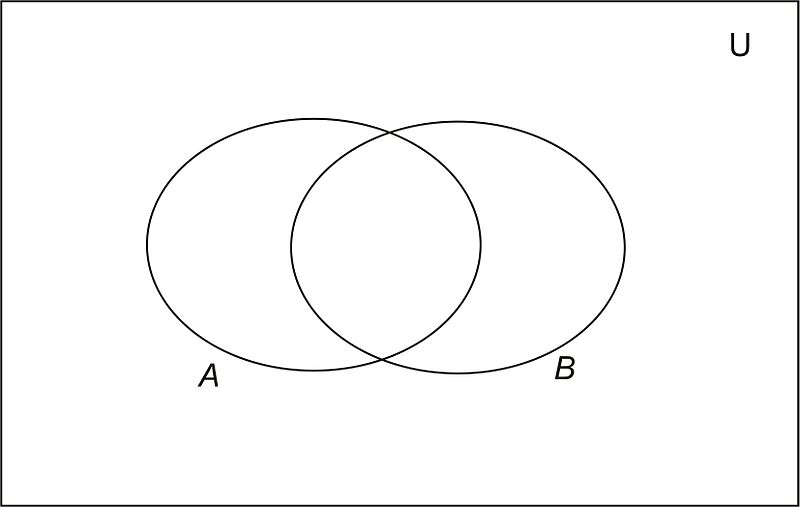
\includegraphics[width=0.8\linewidth]{Venn}
\end{figure}
\end{frame}
%--------------------------------------------------------- %
\begin{frame}
%Question 4
\Large
\[(d) \;\; A^\prime\; \cup\; B^\prime; \]
\begin{figure}
\centering
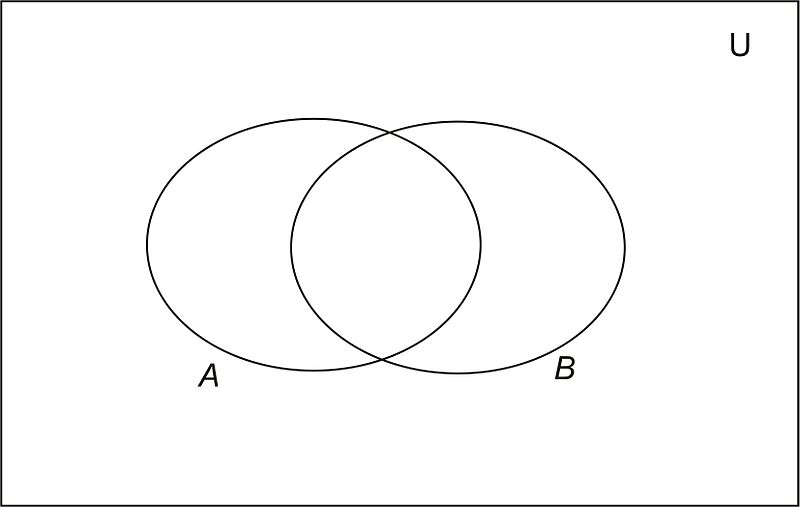
\includegraphics[width=0.8\linewidth]{Venn}
\end{figure}
\end{frame}
%--------------------------------------------------------- %
\begin{frame}
%Question 5
\Large
\[(e) \;\; (A \cup\; B)^\prime;\]
\begin{figure}
\centering
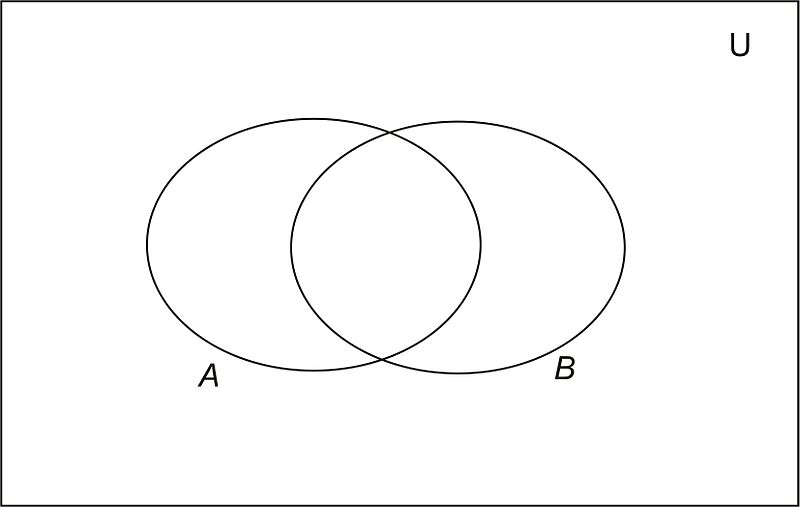
\includegraphics[width=0.8\linewidth]{Venn}
\end{figure}
\end{frame}
%--------------------------------------------------------- %
\begin{frame}
%Question 6
\Large
\[(f) \;\; A^\prime\; \cap\; B^\prime\;\]
\begin{figure}
\centering
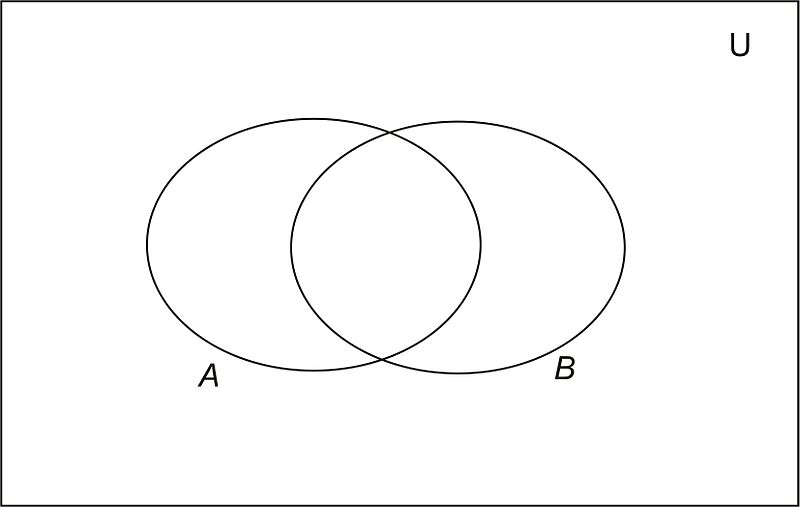
\includegraphics[width=0.8\linewidth]{Venn}
\end{figure}
\end{frame}
%--------------------------------------------------------- %
\begin{frame}
End
\end{frame}
\end{document}
